\subsection{Issue}
Ein \gls{Issue} entspricht im Sinne des Projektmanagements einem Arbeitspaket.
Ein solches \gls{Issue} hat eine Reihe von Eigenschaften oder Attributen.
Diese ermöglichen die Realisierung einer Konvention des Projektmanagement.
Welche dies sind und wie sie genutzt werden, wird im folgenden erläutert.

\subsubsection{Title}
Der \gls{Title} ist die Kurzbeschreibung des \gls{Issue}. Dieser ist kurz und
prägnant gehalten und gibt eine grobe Angabe über dessen Inhalt. Im Kontext
des Projektmanagements stellt dies die Identifikation des Arbeitspakets dar.

\subsubsection{Comment}
Der \gls{Comment} zum Arbeitspaket. Hierbei gibt es zwei Arten von
\gls{Comment} die es zu unterscheiden gilt:

\begin{itemize}
	\item Initialier \gls{Comment}
	\item Alle anderen \gls{Comment}
\end{itemize}

Der initiale \gls{Comment} stellt eine detaillierte Beschreibung des
\gls{Issue} dar, so wie dies auch für das Projektmanagement genutzt wird.
Alle anderen \gls{Comment} bilden ein chronologisch geordnetes Forum,
welches eine detaillierte, transparente und allen zugängliche Historie der
Abwicklung bereitstellt. Dies ist insbesondere wichtig bei der Änderung der
Zuständigkeit. Mit Hilfe dieser Historie kann sich ein Nachfolger schnell
selbstständig einarbeiten. Wesentlich ist hierbei, dass dies Art und Weise
der Erfassung einfach, effizient und demzufolge rege Anwendung findet. Ein
Beispiel ist in der Abbildung \ref{fig:comment} gegeben.

\subsubsection{Status \& Event}
Ein \gls{Issue} hat einen definierten zeitlichen Startpunkt, welcher durch
seinen Instanzierungszeitpunkt gegeben ist. Eine existenzielle
Terminierung ist hingegen nicht vorgesehen. Der Lebenszyklus eines
\gls{Issue} ist nicht abgeschlossen, hat also nur einen definierten Anfang
und kein Ende seiner Lebenszeit.

\begin{figure}[h!]
	\centering
	\begin{tikzpicture}[node distance=2.85cm,scale=0.75,transform shape]
		\node (start) [flowchart-block] {issue is created};
		\node (open) [flowchart-block, right of=start] {issue is open};
		\node (closed) [flowchart-block, right of=open] {issue is closed};
		\draw[->, thick, blue] (start) -- node[anchor=south] {open} (open);
		\draw[->, thick, blue] (open) -- node[anchor=south] {close} (closed);
		\draw[->, thick, blue] (closed) -- ++(2,0) -| node[anchor=south] {reopen} ++(0,-2) -| (open);
		\draw[->, thick, dotted, red] (closed) ++(2,0) -- ++(2,0) node[anchor=west] {issue at end of life};
	\end{tikzpicture}
	\caption{Lebenszyklus eines issue}
\end{figure}

Während dieses Lebenszyklus können verschiedene \gls{Event} auftreten.
Diese sind zwischen den \gls{Comment} dargestellt und somit ebenfalls
chronologisch geordnet. Mögliche \gls{Event} sind dabei

\begin{itemize}
	\item close (\emph{Abschluss})
	\item reopen (\emph{Wiedereröffnung})
	\item assignment (\emph{Änderung der Zuständigkeit})
	\item label (\emph{Änderung der Markierung})
\end{itemize}

Diese \gls{Event} tragen wesentlich zur Transparenz der Abwicklung bei, an
welchem sich alle Projektteilnehmer orientieren können.

\subsubsection{Label}
Das \gls{Label} eines \gls{Issue} ist eine prägnante Markierung, welche mit
Text und Farbe eine Klassifizierung des \gls{Issue} darstellt. Diese können
laufend angepasst und ergänzt werden im Verlauf des Projekts. Die Abbildung
\ref{fig:labels} zeigt eine Liste von \gls{Label}, so wie diese auf GitHub
abgerufen werden kann.

Im Kontext des Projektmanagements stellt das Label ein Hilfsinstrument dar,
welches die lockere Gruppierung von Arbeitspaketen ermöglicht.
Einem Arbeitspaket können dabei mehrere Markierungen zugeordnet werden, wobei
ein übermässiger Einsatz dem Zweck gegenüber als diametral zu betrachten ist.
GitHub unterstützt die Mehrfachmarkierung. So kann ein \gls{Issue}
beispielsweise als \emph{Task für den Bereich der Elektrotechnik} markiert
sein mit dem \gls{Label} ``ET-Task'' als auch \emph{Task betreffend der
Dokumentation} mit dem \gls{Label} ``documentation''.

\begin{figure}[h!]
	\centering
	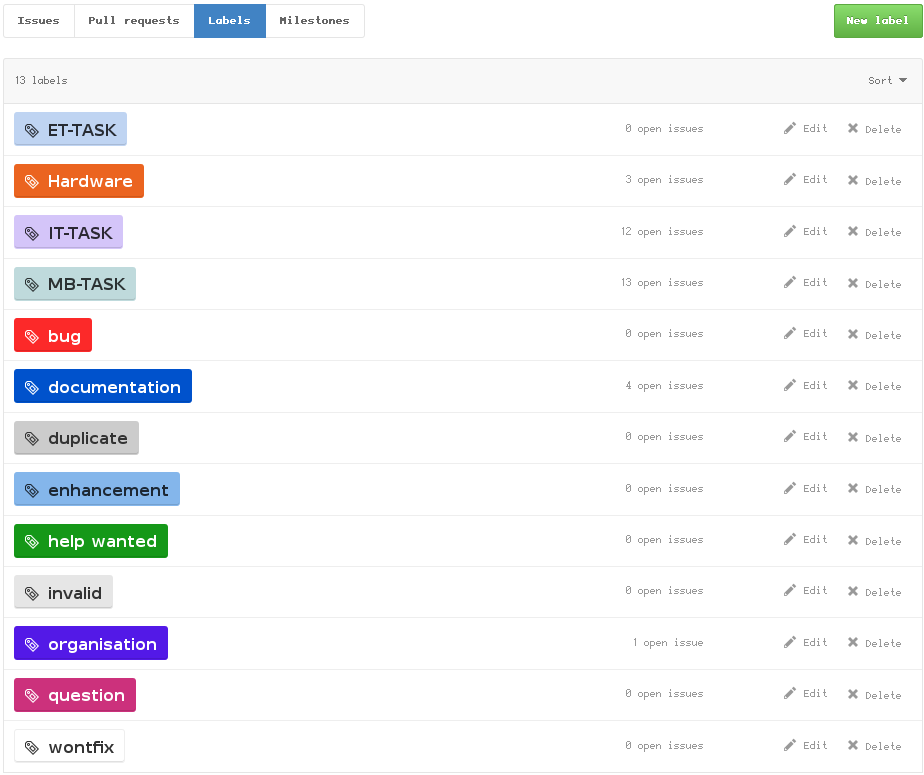
\includegraphics[width=0.75\textwidth]{../../fig/github/labels.png}
	\caption{Übersicht der Labels von \url{github.com/accefa/pren2}}
	\label{fig:labels}
\end{figure}

\subsubsection{Milestone}
Ein \gls{Issue} kann zu einem \gls{Milestone} gelinkt werden. Im Sinne des
Projektmanagement bedeutet dies, dass das \gls{Issue} dem angegebenen
\gls{Milestone} zugehörig ist. Somit ist der Abschluss des \gls{Issue}
eine zwingende Bedingung zur Erfüllen des \gls{Milestone}.

\clearpage
\subsubsection{Beispiel}
Das folgende Beispiel stellt einen Fall dar, welcher nicht dem angestrebten
Arbeitsprozess entspricht, wie dieser in der Abbildung \ref{fig:process}
dargestellt ist. Bei diesem Beispiel ist ein \gls{Issue} erstellt worden ohne
die Angabe eines \gls{Assignee} und \gls{Label}. An genau solch einem
suboptimalen Fall für das Projektmanagement soll gezeigt werden, wie die
Instrumente von GitHub helfen den erfolgreichen Projektfluss aufrecht zu
erhalten. 
\begin{comment}
Hierzu ist in der Abbildung \ref{fig:comment} der Ausschnitt aus der
Anfangsphase solch eines \gls{Issue} dargestellt.
\end{comment}

\begin{figure}[h!]
	\centering
	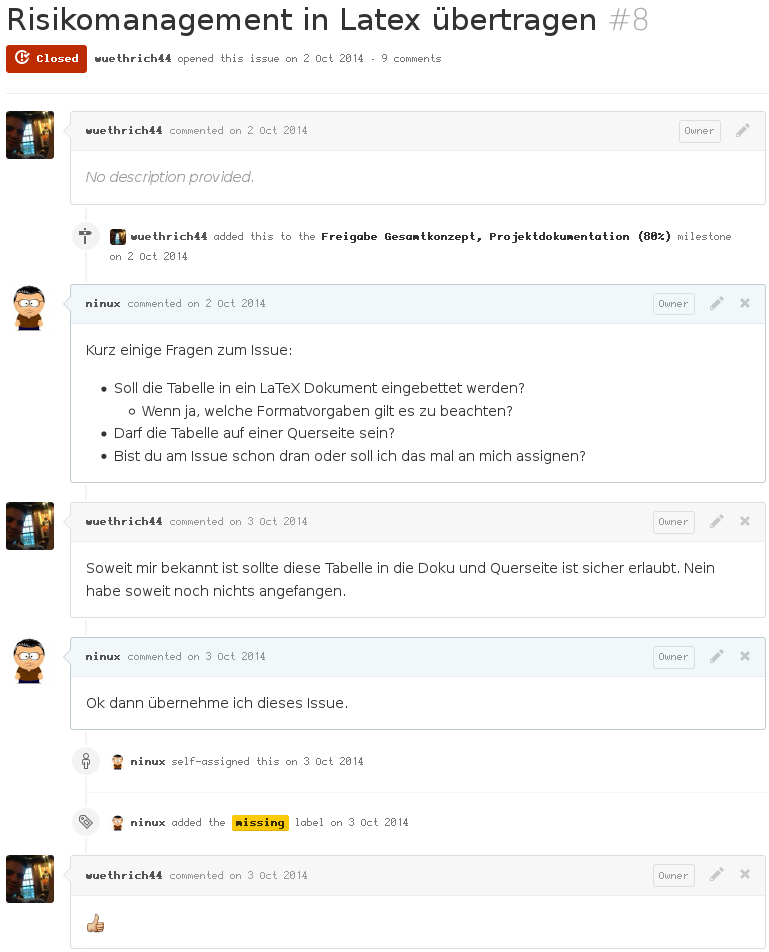
\includegraphics[width=0.75\textwidth]{../../fig/github/issue_comment.png}
	\caption{Ausschschnitt aus der Historie eines Issues}
	\label{fig:comment}
\end{figure}

Im gezeigten Beispiel aus der Abbildung \ref{fig:comment} ist zu erkennen,
dass das \gls{Issue} zunächst einem Meilenstein zugewiesen wird
(\emph{Freigabe Gesamtkonzept, Projektdokumentation (80\%)}). Danach findet
eine Diskussion statt zur Klärung inhaltlicher Fragen zum \gls{Issue}. Diese
führt dann dazu, dass ein Projektteilnehmer zum \gls{Assignee} wird. Dieser
setzt im Anschluss noch ein \gls{Label}. Der daraus resultierende Verlauf ist
eine prägnante Dokumentation für alle Projektteilnehmer, welche sich
jederzeit nachvollziehen lässt.
